\documentclass[a4paper,12pt]{report}

\usepackage{alltt, fancyvrb, url}
\usepackage{graphicx}
\usepackage[utf8]{inputenc}
\usepackage{float}
\usepackage{hyperref}

\usepackage[italian]{babel}

\usepackage[italian]{cleveref}

\title{Relazione \\``Unibomber''}

\author{Riccardo Moretti \\ Alex Tamagnini \\ Niccolò Bertozzi \\Lorenzo Rigoni}
\date{10 aprile 2023}


\begin{document}

\maketitle

\tableofcontents

\chapter{Analisi}

\section{Requisiti}
Il progetto si pone l’obiettivo di creare un videogioco arcade PvE ispirato a “Bomberman”. Con arcade si intende una categoria di videogiochi generalmente frenetici e basati su partite relativamente veloci. Nello specifico un PvE invece è un videogioco basato sull’ affrontare dei nemici gestiti dal computer, che noi chiameremo bot, che generalmente operano su regole di gioco equivalenti a quelle del player umano.

\subsection*{Requisiti funzionali}
\begin{itemize}
    \item Il gioco si occupa di gestire la partita dell’utente all’interno di una mappa scelta in precedenza con un dato numero di bot avversari.
    \item Prima dell’inizio della partita vera e propria sarà possibile scegliere la mappa di gioco, le regole di partita e dei relativi handicap, rendendo dunque i bot più o meno minacciosi verso il player.
    \item Player e bot sono in grado di muoversi, piazzare bombe e raccogliere Power Ups. Se una bomba esplode nelle loro vicinanze vengono eliminati dalla partita. I Power Ups vengono rilasciati a random quando un muro viene distrutto da una bomba.
    \item Quando tutti i bot o il player vengono eliminati si ha, rispettivamente, una vittoria o una sconfitta.
    \item Il gioco si assicura che non si verifichino situazioni di stallo gestendo un “hurry up”, ovvero una fase dove il campo si restringe forzando un conflitto diretto.

\end{itemize}

\subsection*{Requisiti non funzionali}
\begin{itemize}
    \item L'obiettivo del gioco è quello di offrire un'esperienza fluida e gradevole, perciò sarà necessario mantenere prestazioni efficienti.
    \item Il gioco deve essere facile da utilizzare, con un'interfaccia intuitiva.
    \item Il gioco deve mantenere un’ estetica accattivante e colorata come il gioco originale.
\end{itemize}
\newpage
\section{Analisi e modello del dominio}
Unibomber dovrà garantire la possibilità di creare partite tramite un'interfaccia grafica. In particolare, sarà possibile aggiungere o rimuovere una serie di bot che competono tra loro e con il giocatore stesso. In fase di selezione, sarà inoltre possibile scegliere la mappa di gioco, ovvero l'ambientazione in cui si svolge la partita. Intoltre l'utente potrà aggiungere degli handicap, ovvero power up aggiuntivi per i bomber, ovvero player o bot; in modo tale da rendere o più difficoltoso vincere per l’utente, o facilitarlo assegnandosi degli handicap.
\\
Una volta che la partita è iniziata, i bot e il giocatore possono muoversi liberamente, con il giocatore che utilizza la tastiera del proprio dispositivo per spostarsi e piazzare bombe.
Le bombe piazzate esplodono dopo un tempo predeterminato, distruggendo tutti i muri distruttibili e i power up presenti nell'area di effetto e eliminando i bomber che si trovano al suo interno. Il raggio d'azione della bomba è determinato dal numero di power up FIREUP raccolti dal giocatore che ha piazzato la bomba, con un raggio d'azione iniziale di 1.
\\
A meno che non si giochi in mappe prive di muri, il giocatore dovrà utilizzare le proprie bombe per farsi strada e raggiungere gli altri bomber presenti in gioco. Le bombe piazzate dai bomber distruggono tutte le entità con cui entrano in contatto, ma l'esplosione viene bloccata dai muri e dai power up, che vengono distrutti senza essere influenzati dalla fiammata.
\\
Ciò significa che i muri e i power up possono proteggere un bomber che si nasconde dietro di essi. Al contrario, l'esplosione delle bombe non viene bloccata dai bomber e li elimina se si trovano nell'area di effetto.
\\
Se una bomba esplode e colpisce un'altra bomba, questa esplode automaticamente, indipendentemente dal tempo rimanente prima della sua esplosione. L'unica entità non influenzata dall'esplosione della bomba è il muro indistruttibile, che blocca la fiammata ma non viene distrutto.
\\
Ci sono due power up speciali che permettono al giocatore di interagire con le bombe in modo molto vantaggioso: il KICKBOMB consente di spingere una bomba a contatto, mentre il THROWBOMB consente di lanciare una bomba appena piazzata, a patto che il giocatore non si sia ancora allontanato da essa.
\\
Le bombe avranno una fase iniziale in cui non saranno "solide", consentendo al giocatore che le ha piazzate di muoversi liberamente. Tuttavia, una volta usciti dalla bomba, il giocatore perderà questo privilegio e la bomba agirà come un muro solido. In pratica, le bombe avranno due stati fisici: uno "attivo" e uno "passivo", e il giocatore dovrà fare attenzione a non rimanere intrappolato tra le proprie bombe e i muri solidi della mappa.
\\
I power up potranno essere ottenuti fin da subito grazie alle specificità della mappa scelta o facendo esplodere i muri distruttibili lungo la mappa. Quando un muro distruttibile viene distrutto, ha la possibilità di rilasciare un power up. Ci saranno power up basici, che forniranno miglioramenti o peggioramenti alla potenza, al numero di bombe o alla velocità del player, e power up complessi, che offriranno cambiamenti radicali nel modo in cui il bomber interagisce con le altre entità. I power up potranno essere raccolti semplicemente collidendo con essi. Tuttavia, i power up complessi saranno molto più rari da trovare rispetto ai power up basici.
\\
Le bombe sono le armi utilizzate sia dal giocatore che dagli avversari per distruggere i muri e gli avversari. Quando una bomba esplode, causa danni a tutti gli oggetti e ai personaggi presenti nell'area di esplosione.
\\
I muri sono gli ostacoli presenti nell'ambiente di gioco. Possono essere distrutti dalle bombe e possono nascondere dei power up.
\\
I power up sono oggetti speciali che il giocatore può raccogliere per aumentare la forza delle bombe o la velocità di movimento.
\\
Difficoltà:
\begin{itemize}
    \item Un’implementazione di una intelligenza artificiale, intesa come azione/reazione logica allo stato attuale delle entità in gioco, capace di mettere in difficoltà il player umano.
    \item Una grafica completa di animazioni che racchiuda lo stile nostalgico del gioco.
\end{itemize}

\begin{figure}[H]
    \centering{}
    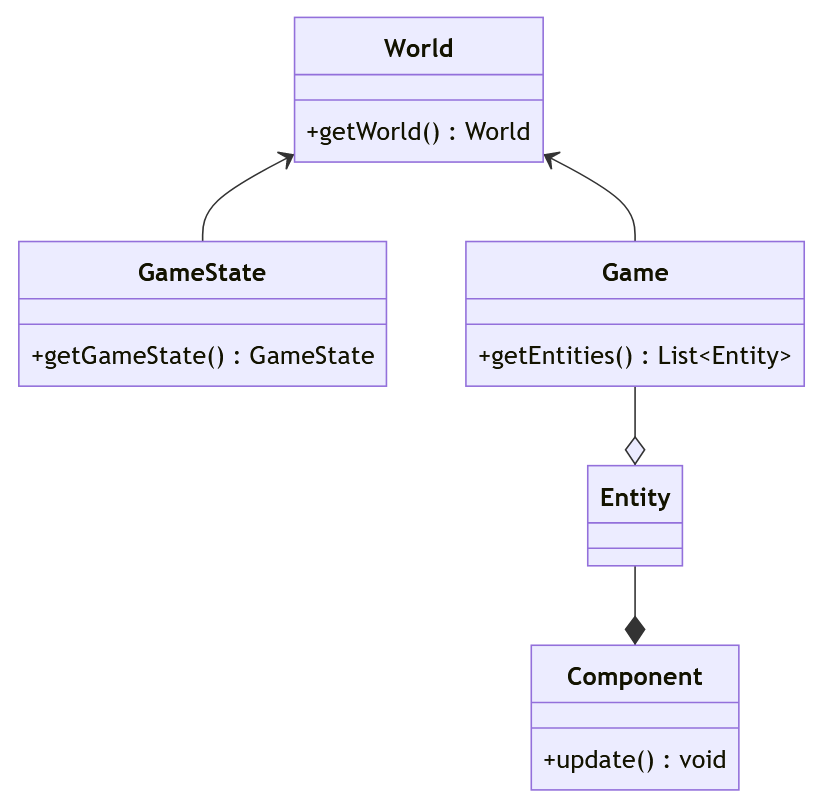
\includegraphics[width=1\textwidth]{img/UMLAnalisi.png}
    \caption{Schema UML delle entità principali}
\end{figure}


\chapter{Design}
\section{Architettura}
Il pattern principale su cui è basato Unibomber è un simil MVC, ovvero divisione del progetto in model view e controller, al quale è stato scelto di accostare l'approccio di sviluppo ECS.
\\
Quest’ultimo, infatti, ci ha permesso di dividere i domini del gioco in sotto-domini più semplici da gestire, rendendo agevolato il Model del progetto e più trasparente la gestione delle entità.
\\
In quest’ottica, ogni entità presente nel gioco apparterrà nominalmente alla stessa classe e le sue peculiarità verranno evidenziate dalle componenti funzionali a loro attaccate (Input, Movimento, collisioni…). La gestione effettiva delle Component è affidata al System, ovvero una sottoparte del controller che si occupa di aggiornare, secondo specifici criteri, le varie Component per evitare conflitti tra di loro o desincronizzazioni.
\\
L’uso delle componenti ci ha portato due grandi vantaggi:
\begin{itemize}
    \item \textbf{Riuso del codice}: avere delle componenti che descrivono ogni dominio ci ha permesso di utilizzarle per più entità diverse tra loro ma con domini presentati intersezioni.
    \item \textbf{Assenza di ereditarietà multiple}: ogni entità è assestante, l’unica ereditarietà gestita è quella delle componenti a una sola classe generale.
\end{itemize}

Riguardo al pattern architetturale Model/View/Controller, la divisione è stata effettuata come segue:
\begin{itemize}
    \item \textbf{Model}: La parte dell’applicativo che rappresenta il Model è contenuto nella cartella Game, come specificato sopra qui vi è presente anche la cartella ecs in cui sono modellate tutte le componenti utilizzate nel progetto. E’ presente un Model per ogni stato del gioco, in modo tale da differenziare i relativi dati ottenendo una struttura molto più ordinata. All’interno della parte Model sono contenuti i dati e la logica base dell’applicazione, i quali cambieranno in runtime durante la partita.
    \item \textbf{View}: Il ruolo della view non è nient'altro che “disegnare” a video i dati relativi ai diversi Model. In base allo stato del gioco (es. MENU, OPTION, PLAY) verrà disegnata la view corrispondente.
    \item \textbf{Controller}: Il controller è colui che metterà in comunicazione il model con la view. In base al GameState il Model aggiornerà i suoi dati runtime; il controller relativo a quel GameState avrà il compito di avvisare la view dei relativi cambiamenti dei dati in modo tale che la view possa poi disegnare in modo corretto.
\end{itemize}
Dal diagramma delle classi, qui sotto fornito, è possibile vedere come abbiamo inserito il pattern MVC all’interno della nostra applicazione.
\\
Come si può notare, la nostra struttura si centra su un controller generale ovvero WordImpl il quale ha il compito di gestire principalmente il Game Loop dell'applicazione.
\\
Inoltre in base al Gamestate il controller World andrà a richiamare i relativi controller dei vari stati di gioco i quali poi andranno a comunicare con i rispettivi Model e View.
\\
Questa suddivisione, organizzata, della struttura offre l'opportunità in una versione futura dell’applicazione di poter cambiare il motore grafico senza estreme difficoltà; andando semplicemente a modificare solo parte di view.
\begin{figure}[H]
    \centering{}
    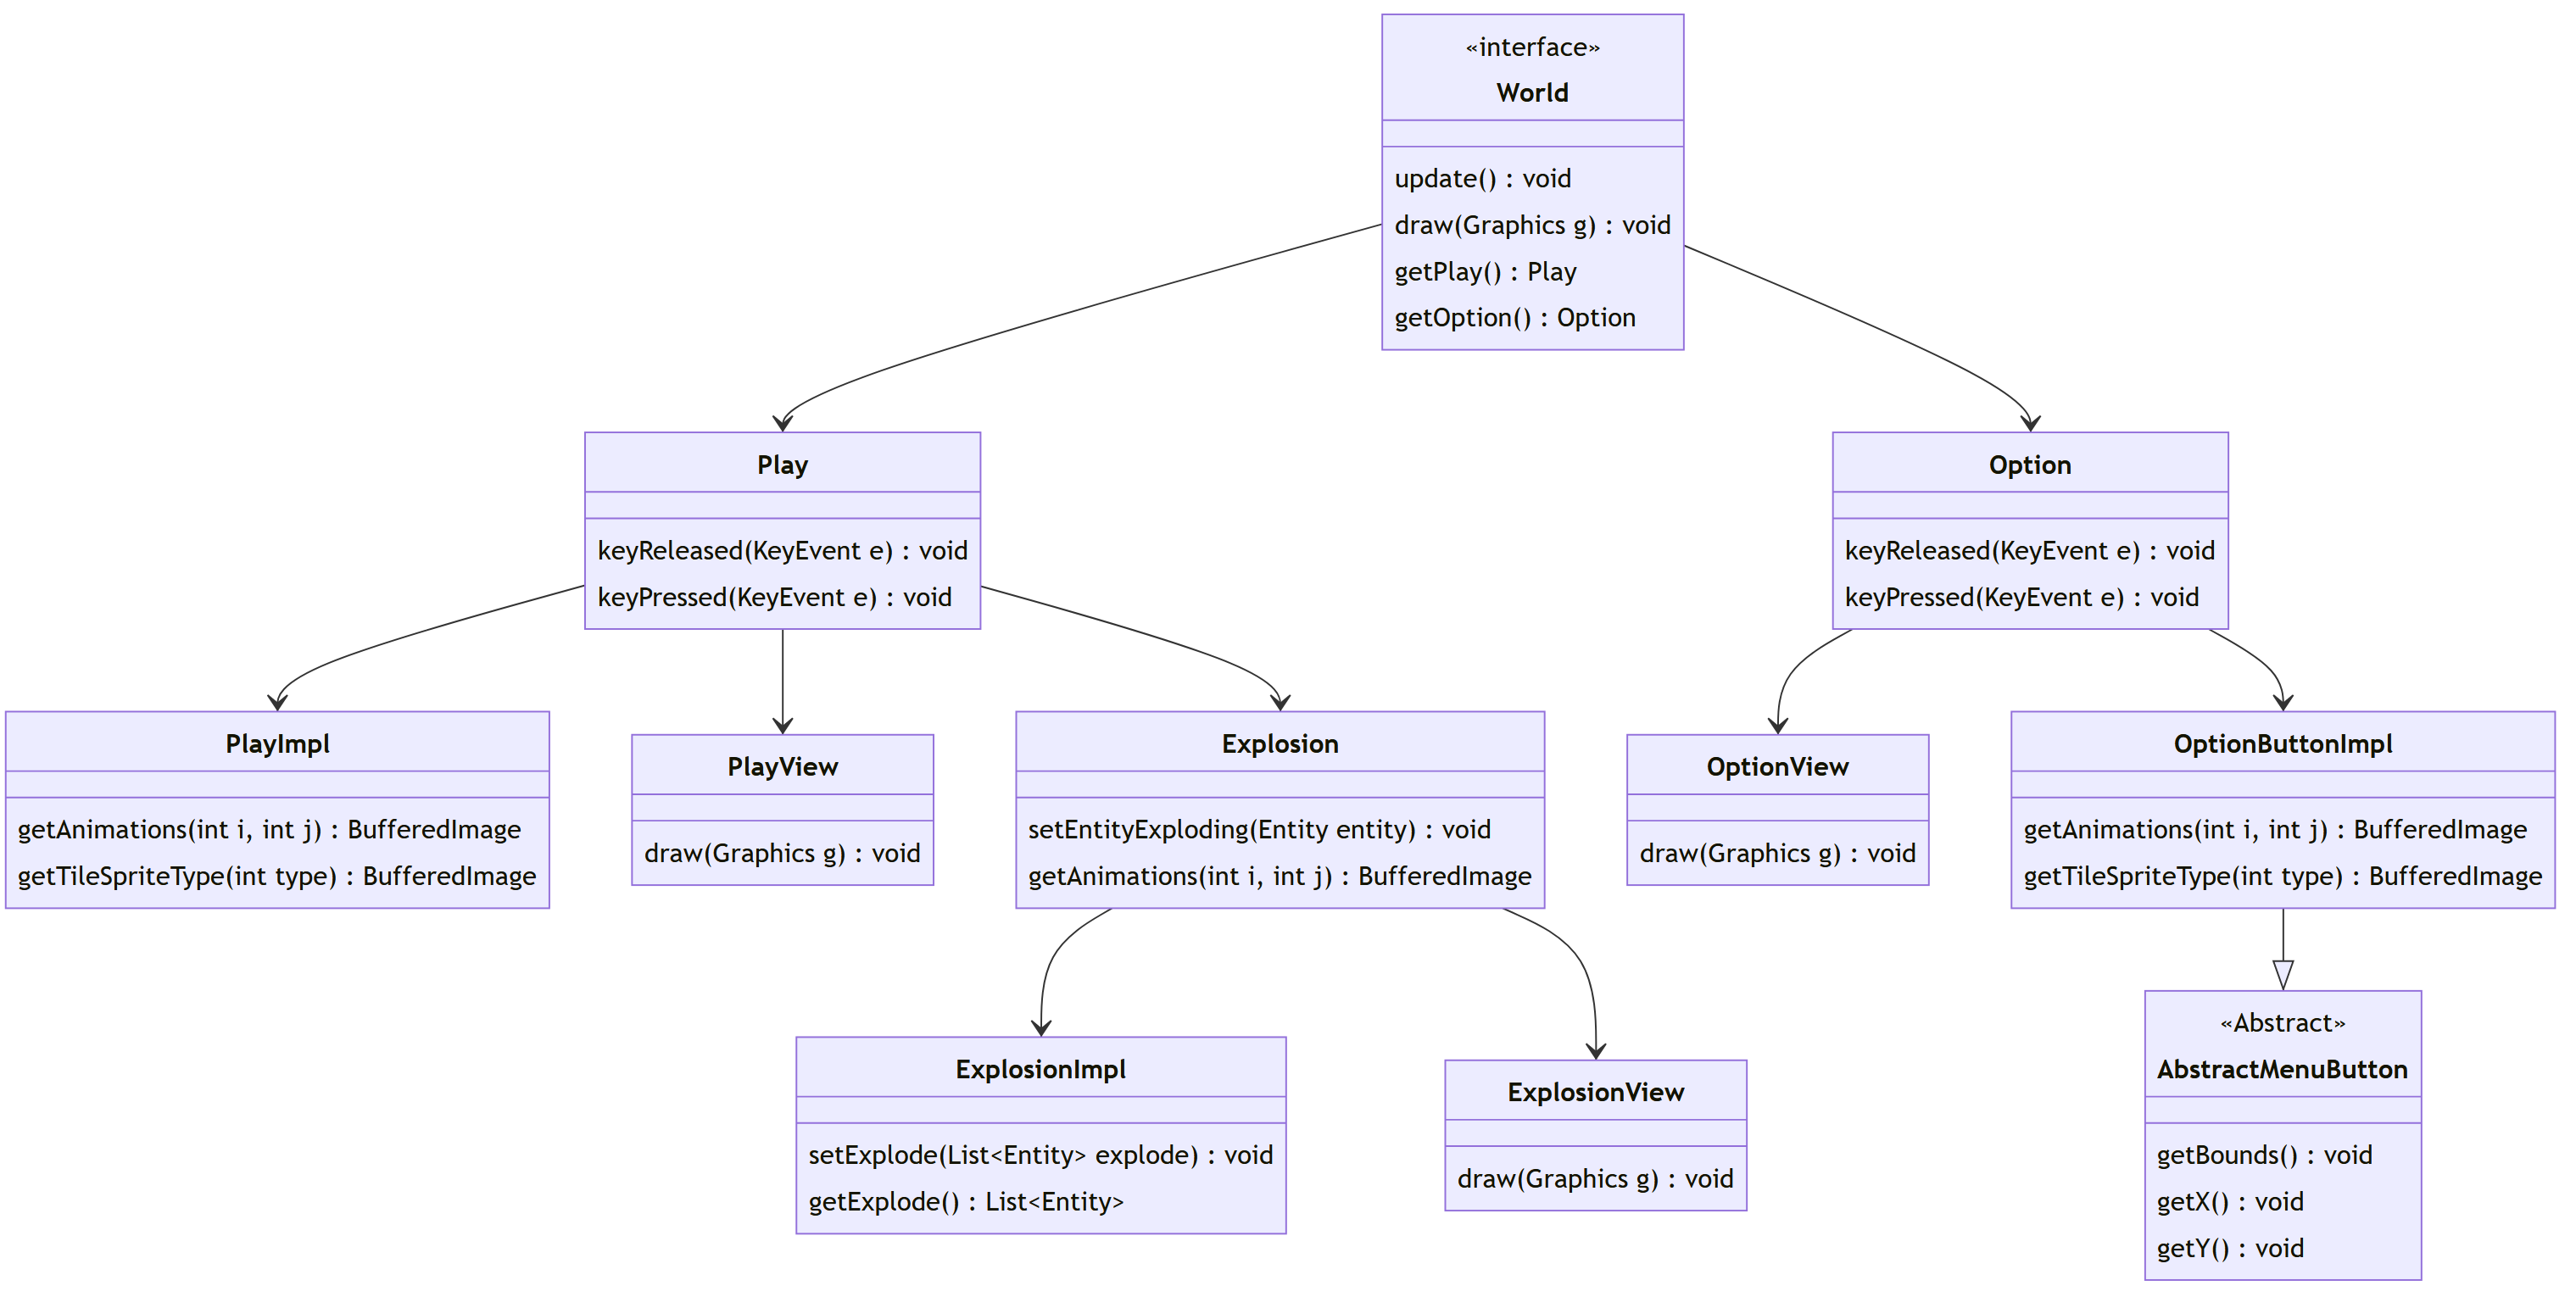
\includegraphics[width=1\textwidth]{img/UMLMVC.png}
    \caption{Schema UML della struttura MVC ,
    NOTA: sono mostrate solo la struttura di Play, Menu e Explosion ma lo schema è equivalente per i restanti controller.}
\end{figure}

\section{Design dettagliato}
%
\subsection*{Riccardo Moretti}
%
\subsubsection*{Separare il dominio del GameLoop da quello del GameEngine}
%
\begin{figure}[H]
    \centering{}
    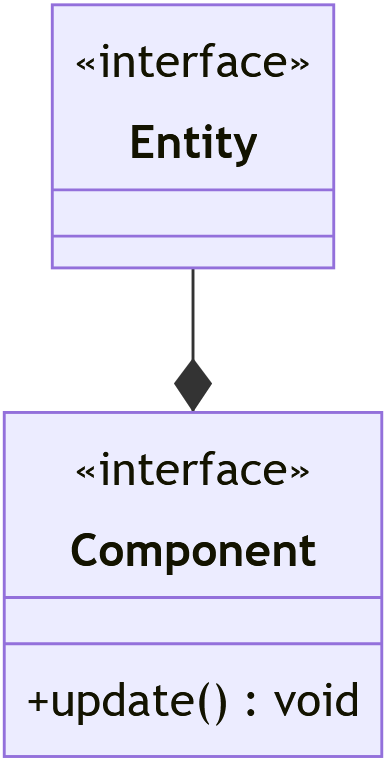
\includegraphics[width=0.4\textwidth]{img/UMLEntita.png}
    \caption{Schema UML dell'oggetto Entity}
\end{figure}
%
\paragraph*{Problema} Diverse istanze di Entity richiedono specifiche che hanno intersezioni tra loro ma rimangono comunque distinte obbligando ad una ripetizione di codice.
\\
Vista la mole di entità concettualmente diverse tra loro, la gestione delle implementazioni di interfaccia potrebbe degenerare in un abuso dell’ ereditarietà potrebbe degenerare in un abuso di ereditarietà con implementazioni distinte che condividono però porzioni di codice.
%
\paragraph*{Soluzione} la struttura Component del pattern ECS permette di non appesantire la struttura dell’ entità con le proprie specifiche, ma di utilizzare delle componenti come moduli funzionali che descrivano il comportamento dell’entità stessa.
Tale soluzione permette inoltre di rispettare appieno il Single Responsibility Principle. Questo comporta una migliore manutenzione del codice non dovendo provvedere alla modifica di diverse iterazioni della stessa porzione di codice.

%
\subsubsection*{Creazione delle entità}
%
\begin{figure}[H]
    \centering{}
    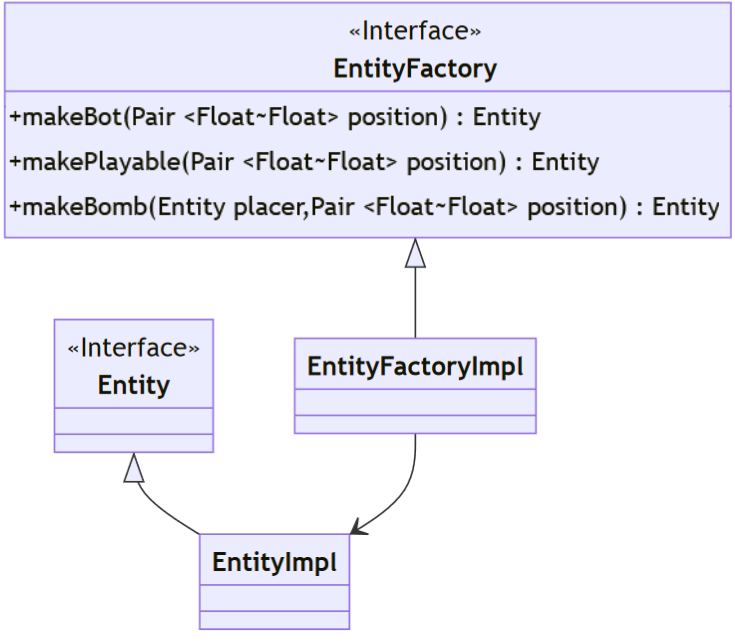
\includegraphics[width=1\textwidth]{img/UMLEntityFactory.png}
    \caption{Rappresentazione UML dello schema di creazione delle entità,
        NOTA: sono mostrate solo tre funzioni nella factory per limiti grafici
    }
\end{figure}
%	
\paragraph*{Problema}  Sarà necessaria la creazione di entità con specifiche diverse con cadenza non unitaria all’interno del progetto.
%
\paragraph*{Soluzione} Per la creazione di entità è stato utilizzato il Factory pattern, un sistema che permette, in questo specifico caso, di centralizzare e unificare il processo in modo da esporre una semplice chiamata all’esterno ogni volta che si renda necessaria la creazione di una specifica entità. La factory crea un layer di
astrazione per la creazione delle entità e nasconde la loro logica di imple-
mentazione. Tramite questo pattern, non sarà  dunque necessario ripetere la prolissa creazione delle varie entità ogni qualvolta sia richiesta la sua creazione.

%
\subsubsection*{Gestione dell'intelligenza artificiale}
%
\begin{figure}[H]
    \centering{}
    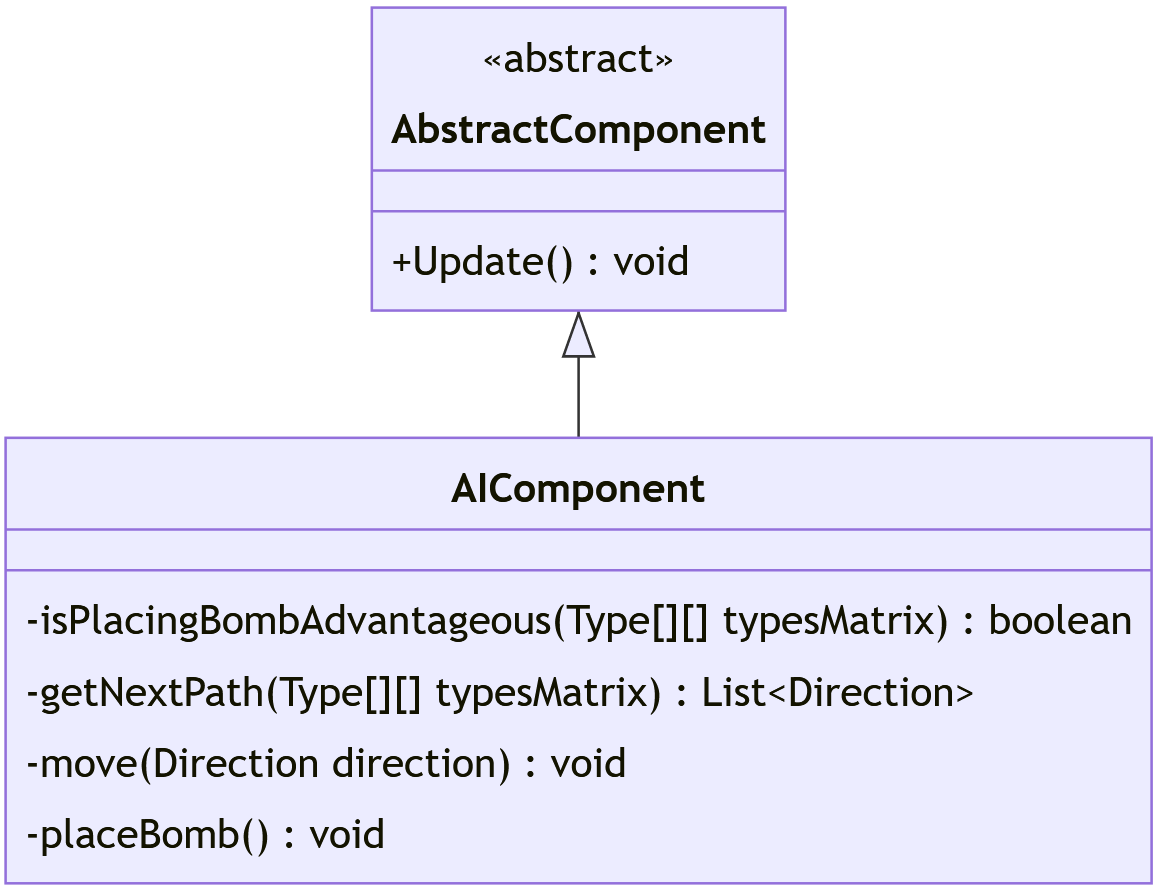
\includegraphics[width=0.75\textwidth]{img/UMLAI.png}
    \caption{Schema UML della gestione dell'AI}
    \label{}
\end{figure}
%
\paragraph*{Problema} Sarà necessaria per i bomber non comandati dal player di poter operare come un giocatore vero, adattandosi alla mappa in cui si trova e decidendo le proprie mosse future in base ai cambiamenti in game.
%
\paragraph*{Soluzione}  Il bot interagisce col mondo tramite una serie di scelte compiute sulla base di una stilizzazione della mappa di gioco, simulata dal parametro typesMatrix che in ogni cella ha un tipo corrispondente ad un’entità in gioco.
In base a ciò che vede controlla innanzi tutto di essere al sicuro da future esplosioni, qualora lo sia decide dove muoversi (prioritizzando la raccolta di power up e l’avvicinarsi a muri ed ad altri Bomber) e se è conveniente per lui piazzare una bomba, tenendo in conto i power up personali.
Il bot cerca di evitare il mettersi in pericolo camminando vicino a bombe in esplosione, ma all stesso tempo può piazzare bombe quando già si trova in range di un esplosione per favorire una reazione a catena, pericolosa per lui, ma anche per ogni Bomber nei paraggi.
Visto l’approccio impiegato per la realizzazione di questa componente, si potrebbe obiettare che il bot non operi su un vero modello di intelligenza artificiale, ma vista la onnipresenza di questo termine in ambito di videoludico come descrittore di comportamenti non determinati dall’input del player ho creduto appropriato scegliere questo nome.

%
\subsubsection*{Gestione del movimento}
%
\begin{figure}[H]
    \centering{}
    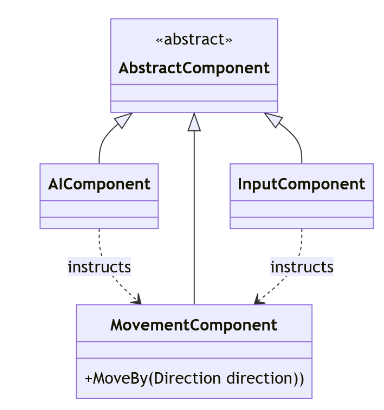
\includegraphics[width=0.75\textwidth]{img/UMLMovement.png}
    \caption{Schema UML della gestione del movimento}
\end{figure}
%
\paragraph*{Problema} Sia bot che player devono poter muoversi tramite azioni (come l’input) per essere scatenate, ma l’evento scatenante è diverso.
La quantità di movimento deve poi essere indipendente dal come la richiesta di movimento sia stata presentata, immaginiamo un frenetico click della chiave di movimento ed una pressione costante.

%
\paragraph*{Soluzione} Divisione della componente di movimento da quelle che lo causano, rispettivamente inputComponent ed AIComponent per player e bot.
La componente di movimento per proteggere se stessa da richieste frenetiche che, se accettate, permetterebbero movimenti illeciti espone un metodo MoveBy che può essere chiamato asincronamente durante la partita passandogli la direzione in cui muoversi, ma l’effettivo spostamento è effettuato ad ogni richiamo del metodo Update (comune a tutte le componenti) e dunque protetto.
La movementComponent gestisce inoltre autonomamente l’applicazione della velocità dell’entità stessa e del moltiplicatore generale di velocità, non ancora utilizzato ma utile per future estensioni.

%%

\subsection*{Lorenzo Rigoni}

\subsubsection{Gestione logica del campo}

\begin{figure}[H]
    \centering{}
    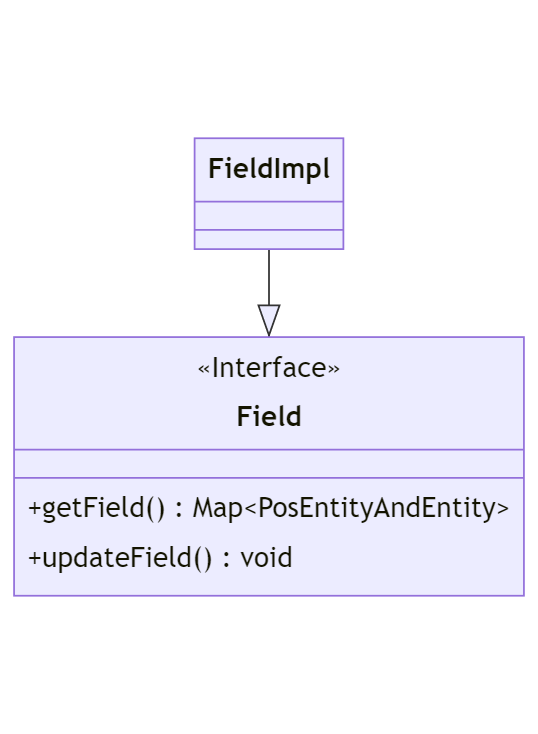
\includegraphics[width=0.50\textwidth]{img/UMLGestioneCampo.png}
    \caption{Schema UML rappresentativo dell'oggetto Field}
    \label{}
\end{figure}

\paragraph{Problema} Ad ogni frame di gioco, il campo subirà delle modifiche e, per questo, ci sarà bisogno di mantenere aggiornate le posizioni delle entità con cui interagisce il player o il bot (i muri, le bombe e i power up).

\paragraph{Soluzione} Dato che ad ogni entità viene associata una posizione del campo, ho optato per la creazione dell’oggetto Field, il quale manterrà le posizioni momentanee delle entità di interesse nel campo e lo aggiornerà ogni volta che viene richiamato.
\\
NOTA: la soluzione del problema è stata fatta con la collaborazione di Moretti Riccardo, in quanto l’oggetto viene molto usato nell’AIComponent da lui svolto.


\subsubsection{Gestione logica dei muri}

\begin{figure}[H]
    \centering{}
    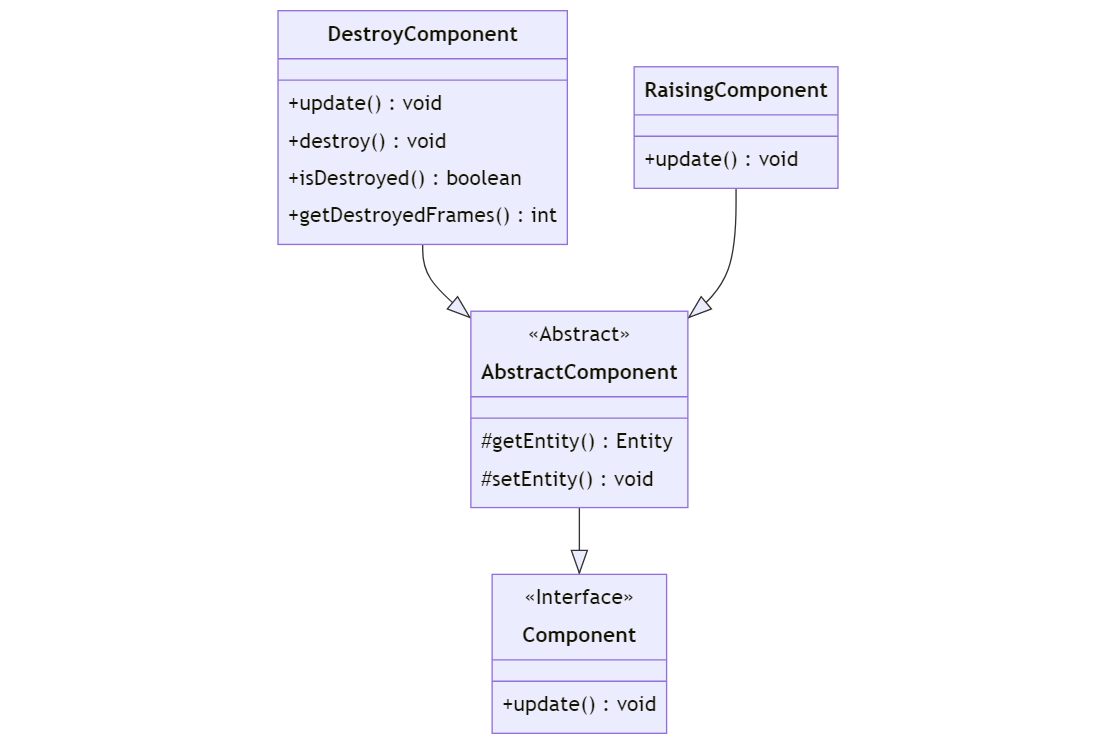
\includegraphics[width=1\textwidth]{img/UMLGestioneMuri.png}
    \caption{Schema UML della gestione logica dei muri}
    \label{img:command}
\end{figure}

\paragraph{Problema} La partita prevede la creazione e gestione di 2 tipi diversi di muro:
\begin{itemize}
    \item Il muro indistruttibile
    \item Il muro distruttibile
\end{itemize}
Inoltre, il muro distruttibile può rilasciare nel campo un power up randomico al momento della sua distruzione.


\paragraph{Soluzione} Per rendere il codice riutilizzabile, ho optato per l’utilizzo del Template Method pattern. Infatti, il metodo template sarà update(), ereditato dalla classe astratta AbstractComponent, il quale verrà implementato dalla componente DestroyComponent per la gestione della distruzione delle entità e (in caso fosse previsto) del conseguente drop del power up in modo randomico.
\\
Inoltre, un altro pattern che ho deciso di utilizzare per creare le entità “Wall” è il Factory method pattern, in modo da semplificare la creazione e una possibile aggiunta futura per quanto riguarda i muri. Inizialmente, avevo creato una classe WallFactory dove, dipendentemente dal tipo di muro, associavo il DestroyComponent oppure no all’entità creata. Successivamente, in base a valutazioni di gruppo, ho deciso di spostare i metodi della WallFactory nella EntityFactory, in modo da avere la creazione di tutte le entità in un’unica factory.
\\
Infine, per rendere più suggestivo il gioco, insieme al gruppo abbiamo deciso di implementare i raising wall, ovvero dei muri indistruttibili che iniziano a comparire attorno al campo restringendolo, alzando così la probabilità di un vincitore piuttosto che un pareggio. Per fare ciò, è stato creato un RaisingComponent seguendo sempre il Template Method pattern.


\subsubsection{Gestione logica della bomba}

\begin{figure}[H]
    \centering{}
    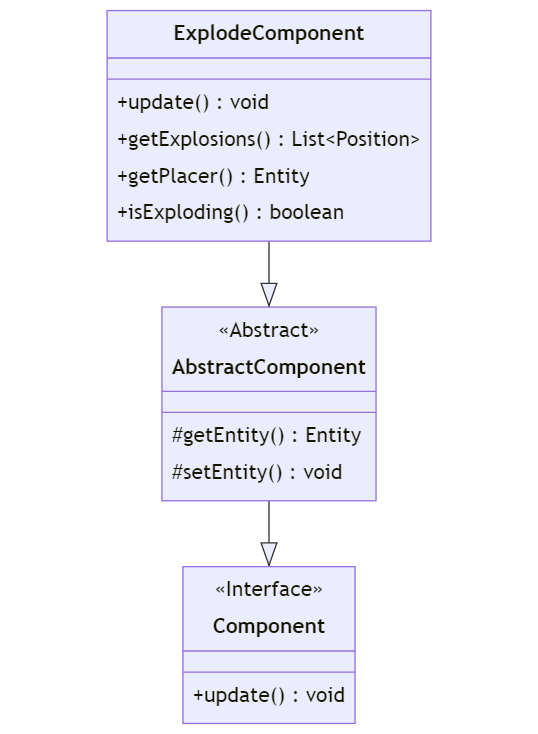
\includegraphics[width=0.75\textwidth]{img/UMLGestioneBombe.png}
    \caption{Schema UML della gestione logica della bomba}
    \label{}
\end{figure}

\paragraph{Problema} Il gioco prevede che il player possa rilasciare delle bombe nel campo. Quest’ultime, hanno il potere di distruggere tutte le entità (tranne i muri indistruttibili) che troveranno nel loro range di esplosione. Inoltre, ogni bomba avrà un tempo di attesa prima di esplodere e una durata dell’esplosione nella quale, ogni entità distruttibile che si troverà all’interno del range della bomba, verrà distrutta.

\paragraph{Soluzione} Come nel caso della gestione dei muri, ho optato per l’uso del Template Method Pattern, ereditando sempre dalla classe AbstractComponent il metodo update, per creare l’ExplodeComponent.
\\
Dunque, ogni bomba ha il proprio ExplodeComponent che gli gestisce, dal punto di vista logico, tutto ciò che deve accadere nel tempo di attesa e durante l’esplosione.
\\
Inoltre, per massimizzare il riutilizzo del codice, tutte le entità nel range della bomba (inclusa la bomba stessa al termine dell’esplosione) vengono distrutte dal DestroyComponent, il quale distrugge tutte le entità in cui viene richiamata la suddetta component.
\\
Infine, anche per l’entità bomba è stato deciso dal gruppo di sviluppare la creazione nella factory “EntitiyFactory”.

\subsection*{Alex Tamagnini}

\subsubsection{Gestione logica dei power up}

\begin{figure}[H]
    \centering{}
    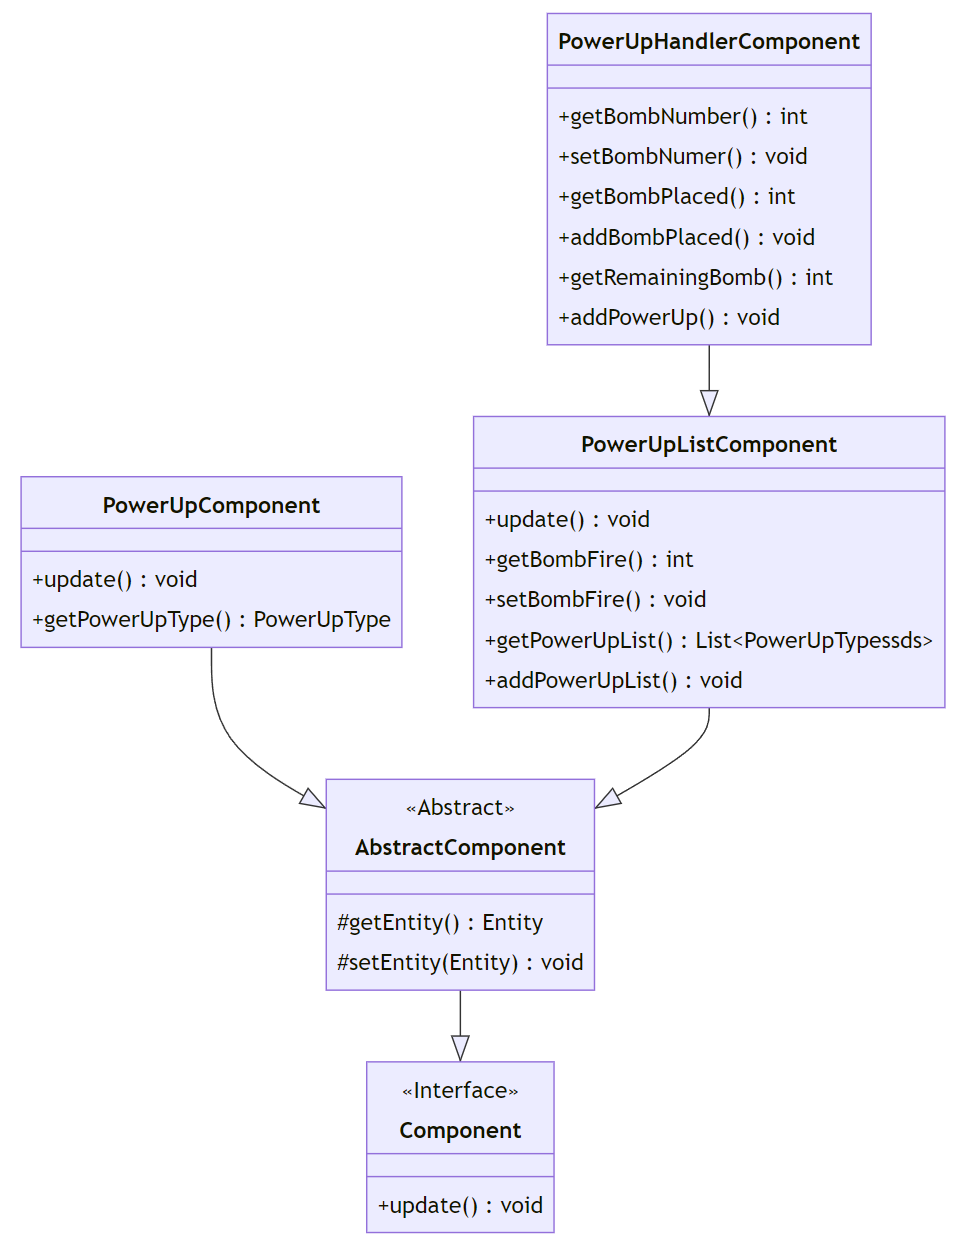
\includegraphics[width=0.90\textwidth]{img/UMLPowerUp.png}
    \caption{}
\end{figure}

\paragraph{Problema} Il player e i bot possono usufruire di eventuali power up, i quali possono modificare la loro velocità, la loro potenza di esplosione e il numero di bombe che possono piazzare. Oltre ad aggiungere due abilità quali calciare la bomba e lanciare la bomba. Anche le bombe devono contenere la potenza di esplosione, inoltre, in una implementazione futura, possono contenere una lista di power up (come ad esempio bomba spinata).

\paragraph{Soluzione} Come prima cosa ho creato un enum che contiene tutti i power up con il rispettivo attributo di complessità. Ho così sviluppato un metodo in grado di ritornare un power up randomico in base alla percentuale di complessità. Ho inoltre implementato un metodo che permette di capire se un power up è positivo o no.
Ho poi creato PowerUpComponent utilizzando Template Method pattern, ereditando  il template update() dalla classe astratta AbstractComponent, il quale rappresenta uno specifico power up che ne ritorna il tipo.
Per quanto riguarda il possedimento di power up per l’entità bomba ho creato PowerUpListComponent, il quale contiene l’attributo potenza bomba e una lista di power up. Ho preso questa decisione in quanto, in vista di future estensioni del codice, è possibile aggiungere power up alla bomba, per modificarne il tipo di esplosione, ad esempio bomba spinata oppure bomba atomica.
Ho poi esteso questa classe creando la componente PowerUpHandlerComponent, la quale è attribuita all’entità bomber. Questa, oltre agli attributi derivati, contiene l’attributo numero bombe disponibili e numero bombe piazzate. All’interno di questa classe è presente un metodo che va a modificare direttamente gli attributi del bomber in base ai power up e controllare il numero di bombe che il bomber può ancora piazzare.
Per quanto riguarda l’attributo speed, per generalizzare la gestione, si trova direttamente nella classe Entity, ma comunque viene modificata dal gestore sopra citato. Anche per questi ultimi ho utilizzato il Template Method pattern con stesse caratteristiche.


\subsubsection{Gestione logica del piazzamento della bomba}

\begin{figure}[H]
    \centering{}
    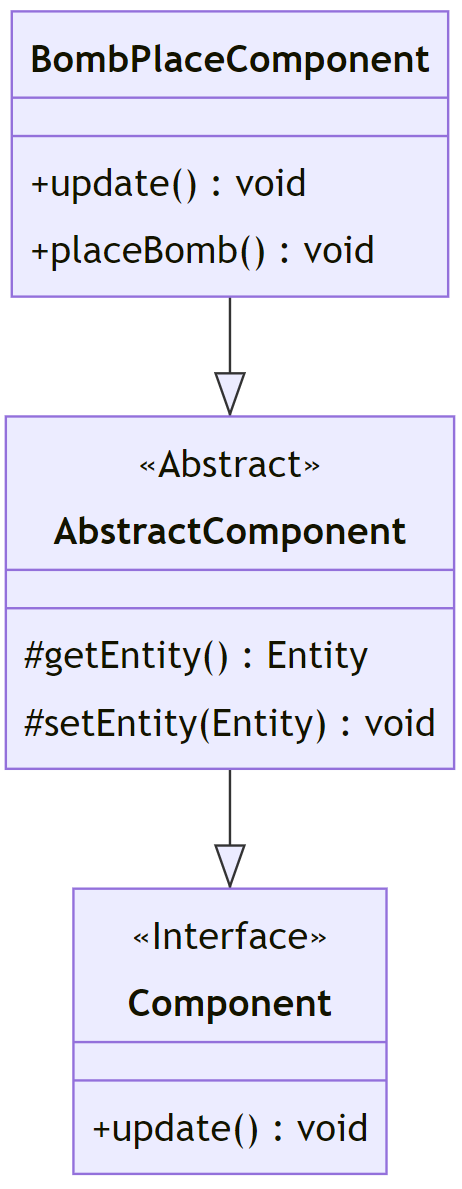
\includegraphics[width=0.4\textwidth]{img/UMLPlaceBomb.png}
    \caption{}
\end{figure}

\paragraph{Problema} Il gioco prevede che il player ed i bot possono piazzare delle bombe nel campo per distruggere muri distruttibili e uccidere nemici.

\paragraph{Soluzione} Per permettere ai bomber di piazzare le bombe ho creato la classe BombPlaceComponent, la quale eredita il metodo template update() dalla classe AbstractComponent, sfruttando il pattern Template Method. Questa classe dunque permette al bomber di posizionare una bomba solo dopo aver cliccato “spazio” ed aver controllato il numero di bombe disponibili, oltre a verificare di non trovarsi su un’altra bomba. Una volta piazzata la bomba, il numero di bombe disponibili viene modificato nel PowerUpHandlerComponent.


\subsubsection{Gestione logica delle abilità speciali del bomber}

\begin{figure}[H]
    \centering{}
    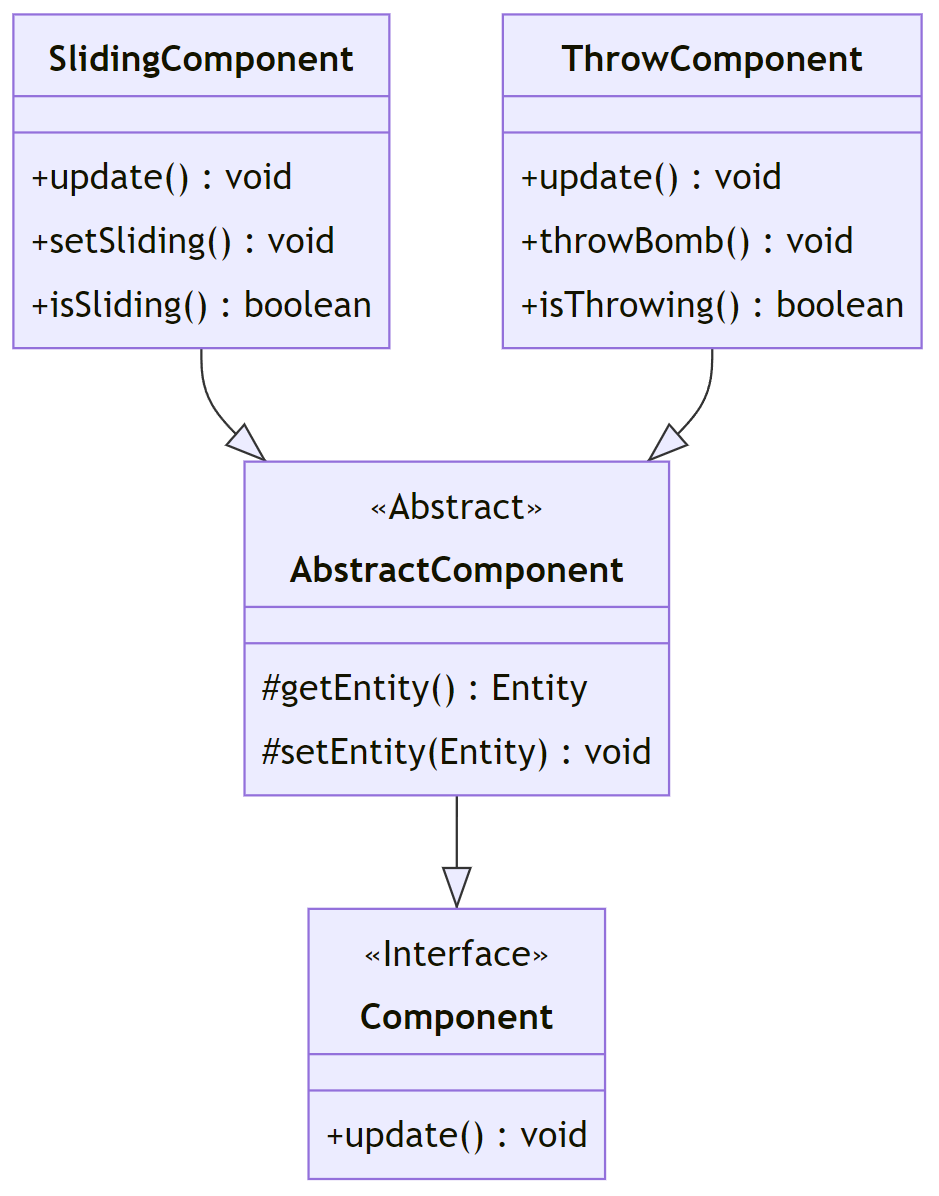
\includegraphics[width=0.5\textwidth]{img/UMLKickThrowBomb.png}
    \caption{}
    \label{}
\end{figure}

\paragraph{Problema}  Il gioco prevede che il bomber, possedendo il corretto power up, può calciare o lanciare la bomba. La bomba può essere calciata in tutte le direzioni e si muove fino a che non esplode oppure entra in collisione con un’altra entità. Per quanto riguarda il lancio invece, questo prevede un lancio in tutte le direzioni, con un raggio standard di 3, con conseguente rimbalzo di 1 fino a che non trova una posizione libera, la bomba può inoltre oltrepassare i bordi esterni e comparire dal lato opposto.

\paragraph{Soluzione} Per permettere alla bomba di essere calciata, come prima cosa viene controllata la collisione tra bomber e bomba oltre al possedimento del power up KICKBOMB. Successivamente viene richiamato SlidingComponent, all’interno del quale, grazie alla direzione del player, richiamo il MovementComponent che permette alla bomba di muoversi, fino a che non entra in collisione con un muro, un altro bomber oppure un’altra bomba, a questo punto viene fermato il metodo update di SlidingComponent. Se nel suo percorso incontra altri power up questi vengono distrutti.
L’abilità del lancio della bomba invece avviene attraverso il click del tasto ‘E’ se ci si trova sopra una bomba appena piazzata e se il bomber contiene il power up THROWBOMB. A questo punto viene richiamato il metodo ThrowComponent che prende posizione e direzione del player, calcolando inoltre la posizione di atterraggio finale standard, quindi di raggio 3. Finché la bomba non si trova nella ipotetica posizione finale, il metodo Update richiama il MovementComponent che permette lo spostamento della bomba. Una volta raggiunta la posizione finale ipotetica, se questa risulta libera da altre entità, viene fermato il metodo Update, altrimenti continua il movimento di un blocco alla volta nella stessa direzione. Ho aggiunto inoltre il controllo che, se la posizione finale risulta fuori dalla mappa, questa viene spostata dalla parte opposta del campo, mantenendo sempre la stessa gittata.
Anche per queste due componenti ho utilizzato il pattern Template Method ereditando il metodo update() dalla classe astratta AbstractComponent.

\subsection*{Niccolò Bertozzi}

\subsubsection{Gestione del ridimensionamento dinamico della finestra di gioco}

\begin{figure}[H]
    \centering{}
    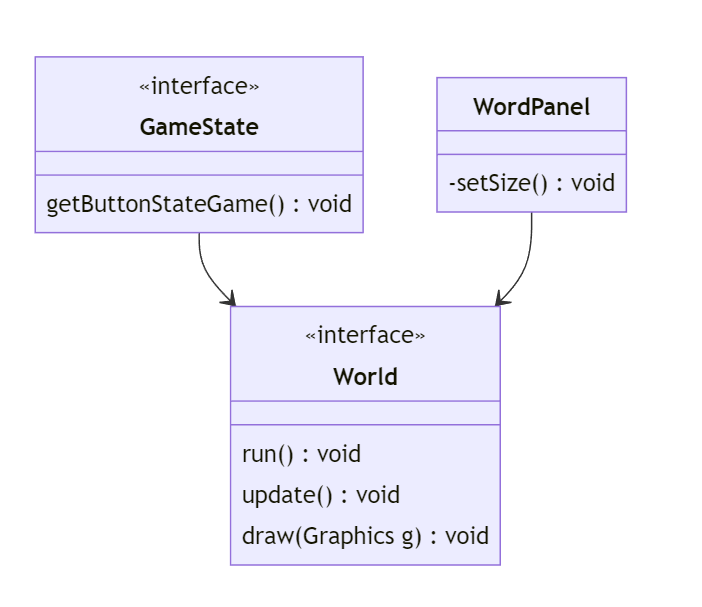
\includegraphics[width=0.75\textwidth]{img/UMLFinestraDiGioco.png}
    \caption{UML struttura finestra di gioco}
\end{figure}

\paragraph{Problema} Ogni utente avrà uno monitor, dove giocherà, differente. Avendo eliminato la possibilità di ridimensionare la finestra occorre ridimensionare correttamente tutte le relative scale grafiche.

\paragraph{Soluzione} Al primo caricamento del gioco verrà creato un JFrame centrato orizzontalmente, mentre verticalmente in base alle dimensioni dello schermo dell’utente verrà inserito in modo tale da occupare il maggior spazio possibile per una giocabilità migliore. Inoltre il SetSize non solo va a ridimensionare la finestra ma va anche a scalare tutti i bottoni e i relativi componenti grafici in modo tale che possano essere visibili alla maggior parte degli utenti.

\subsubsection{Gestione del GameLoop}

\begin{figure}[H]
    \centering{}
    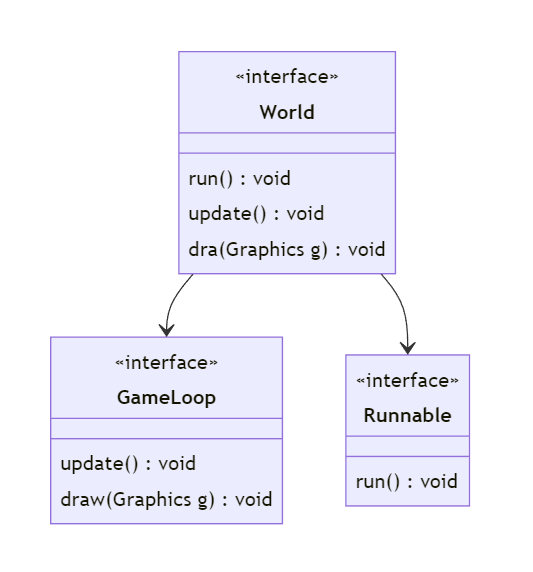
\includegraphics[width=0.75\textwidth]{img/UMLGameLoop.png}
    \caption{UML struttura GameLoop}
\end{figure}

\paragraph{Problema} Il nucleo centrale dell’applicazione è il GameLoop il quale permette di controllare il gioco ad interazioni cicliche di aggiornamenti con una data frequenza. Ad ogni ciclo di frequenza il GameLoop deve essere in grado di aggiornare sia la logica che la grafica dell’applicazione.

\paragraph{Soluzione} Per la gestione del GameLoop viene seguito un tradizionale diagramma a blocchi. All’avvio dell’applicazione, il Controller base del gioco fa partire il Thread, che gestirà il GameLoop. Sono andato a separare l’aggiornamento grafico e quello logico. Per quanto riguarda l'aggiornamento logico, è stato settato un UPS (Update per second) il quale ad ogni ciclo va ad eseguire update logico del relativo gameState che è in corso in quel momento. Per la parte grafica, è stato settato un FPS (Frame per second), il quale però attualmente è libero e questo indica che la parte grafica viene aggiornata frequentemente.

\subsubsection{Gestione logica delle collisioni tra entità}

\begin{figure}[H]
    \centering{}
    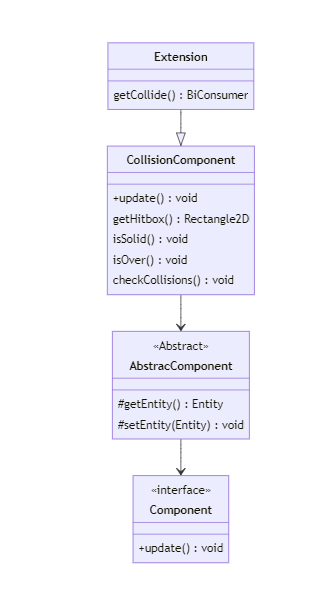
\includegraphics[width=0.75\textwidth]{img/UMLCollisioni.png}
    \caption{UML struttura CollisionComponent}
\end{figure}

\paragraph{Problema}  La gestione delle collisioni delle hitbox delle entità, sapendo appunto anche la tipologia di esse in modo tale da eseguire l’azione corretta. Un’altro problema è la collisione con la bomba in quanto inizialmente il bomber può passare al di sopra di essa, ma una volta uscito dalla sua hitbox non potrà più entrarci.

\paragraph{Soluzione} Come prima cosa, dopo uno studio dell’applicazione originale, ho creato un hitbox (Rectangle) generale per ogni entità (wall, bomber, power up). Una volta create le varie hitbox, ho controllato il flag IsSolid che mi mette in condizioni di sapere se quell’entità è solida (muro) o meno (bomer) e poi tramite un metodo già fornito da Java andavo a verificare se due Rectangle, e quindi appunto due hitbox, stavano collidendo tra di loro. Inizialmente avevo creato tutto all’interno del Collision Component, ma successivamente ad una analisi effettuata con Moretti, per alleggerire il codice e renderlo più leggibile e corretto, siamo andati a crearci una classe specifica che verificava questo ovvero Extension, la quale veniva semplicemente richiamata dalla CollisionComponent passandogli le due entità che collidevano. La classe Extension utilizza l’operatore BiConsumer il quale accetta due argomenti in input e non restituisce alcun risultato. In questo modo abbiamo potuto diversificare le varie entità. In tal modo come primo argomento era presente il soggetto della collisione, mentre come secondo argomento colui che veniva colpito. Facendo così eravamo in grado di conoscere esattamente le due entità e poter quindi successivamente, in base alla collisione che era avvenuta (bomber -> power up, bomber -> wall, bomb -> wall) eseguire la determinata azione necessaria.
Per la gestione della collisione con la bomba inizialmente alla sua creazione viene settata con indice isOver a true, in modo tale che il plater possa collidere con lei senza problema. Ad ogni update il CollisionComponent andrà a verificare se il bomber è ancora all’interno dell’ hitbox della bomba o meno; nel momento in cui uscirà il flag IsOver verrà settato a false e ciò significa che nessuno potrà più entrarci.


\subsubsection{Gestione dei GameState}

\begin{figure}[H]
    \centering{}
    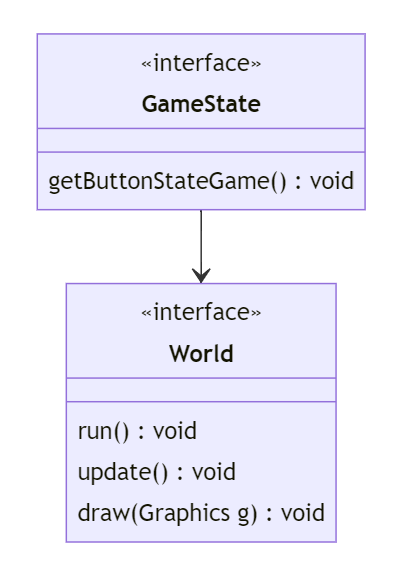
\includegraphics[width=0.75\textwidth]{img/UMLGestioneGameState.png}
    \caption{UML struttura per la gestione degli stati del gioco}
\end{figure}

\paragraph{Problema} In base allo stato del gioco doveva essere messo in esecuzione il controller corretto, il quale andrà poi a disegnare con la relativa view a video tutti i dati offerti dal suo Model.

\paragraph{Soluzione} Il gioco parte di default con il GameState settato su MENU, in questo modo quando l’applicazione verrà caricata per la prima volta verrà visualizzata la schermata di menu in quanto all’interno dei due metodi update e draw di World sarà presente un controllo che in base al GameState andrà a richiamare il controller specifico. All'interno del gioco sarà poi possibile entrare in  pausa e questo andrà a fermare l’applicazione andando anche a stoppare il conteggio dell hurry up finale. In questo modo solo il controller relativo allo stato di gioco corrente verrà richiamato mentre tutti gli altri resteranno in attesa di essere chiamati.

\subsubsection{Gestione del Menu}

\begin{figure}[H]
    \centering{}
    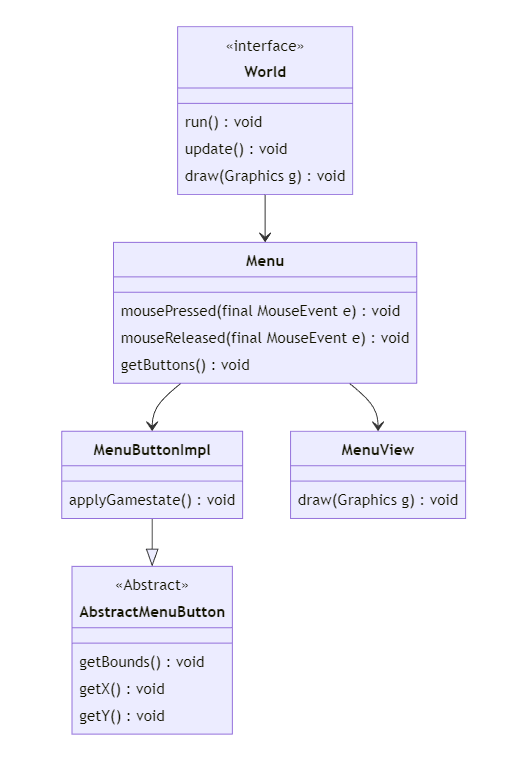
\includegraphics[width=0.75\textwidth]{img/UMLGestioneMenu.png}
    \caption{UML struttura MVC per il menu}
\end{figure}

\paragraph{Problema} Il gioco prevede che durante il menu tu possa iniziare una partita o uscire dal gioco

\paragraph{Soluzione} Il menu è la prima schermata che l’applicazione mostra come prima cosa vengono caricate nel Model tutti gli sprites relativi al background e ai bottoni di scelta in un buffer in modo tale che non dovranno poi essere ricaricati nuovamente. Successivamente il controller del menu nel momento in cui viene richiamato dal Word il quale gli comunica che deve disegnare il menu, provvederà a interpellare la view che disegnerà a video il background e i relativi bottoni di scelta (Battle game, quit).

\subsubsection{Gestione delle opzioni}

\begin{figure}[H]
    \centering{}
    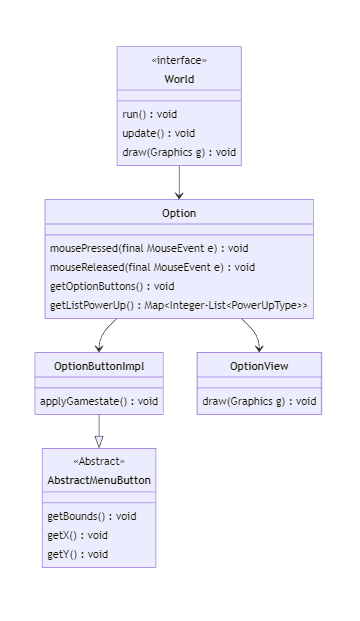
\includegraphics[width=0.75\textwidth]{img/UMLGestioneOpzioni.png}
    \caption{UML struttura MVC per la pagina degli option}
\end{figure}

\paragraph{Problema} Il gioco prevede che si possano settare delle impostazioni di base della partita ovvero scegliere la mappa, indicare contro quanti Bot si vuole giocare e assegnare degli handicap power up al player o ai bot.

\paragraph{Soluzione} Successivamente al menu se l’utente deciderà di effettuare una partita cliccando sul bottone “Battle Game” verrà caricata la schermata di Option la quale permetterà all’utente di settare le impostazioni base di gioco. Come prima cosa l’utente potrà selezionare la mappa che desidera (per i test di consegna saranno caricate due mappe), andando a  sceglierla tramite le due frecce. Subito sottostante sarà disponibile la selezione del numero dei bot, il quale permetterà tramite un semplice click di aumentare (bottone +) o diminuire (bottone -) il numero. Attualmente sarà possibile scegliere da 1 ad un massimo di 3 bot ma tramite l’incremento di una semplice costante sarà possibile aumentare o diminuire il massimo numero di bot presenti nell’arena. Una volta scelto il numero di bot sarà possibile assegnare gli handicap. Basterà cliccare sull'utente a cui si vuole assegnare il power up il quale verrà evidenziato graficamente e successivamente si sceglieranno i power up da assegnare. Sarà possibile, come da gioco originale, assegnare un massimo di sei power up per utente.
Una volta settate tutte le impostazioni basterà cliccare sul bottone “Ok” per poter incominciare a giocare.

\subsubsection{Gestione del gioco}

\begin{figure}[H]
    \centering{}
    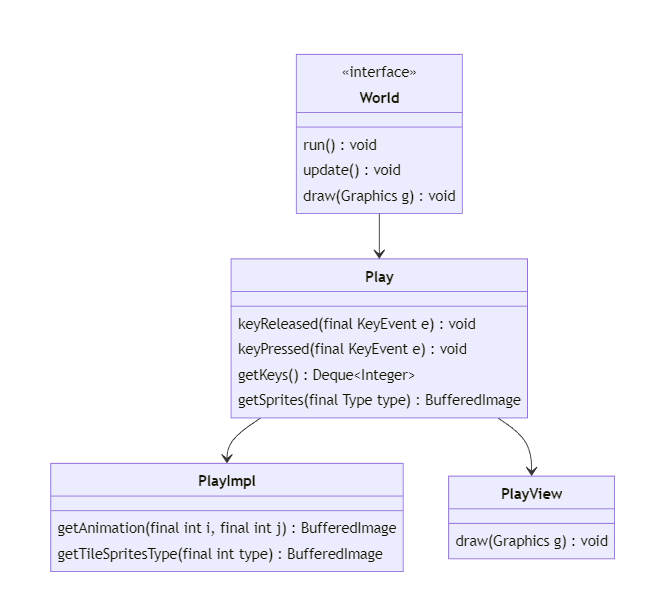
\includegraphics[width=\textwidth]{img/UMLGestioneGioco.png}
    \caption{UML struttura MVC per la gestiona della partita}
\end{figure}

\paragraph{Problema} In base alla frequenza del GameLoop il gioco dovrà aggiornare i dati e la grafica in modo fluido e gradevole all’utente. Inoltre nel caso in cui avvenga una perdita di prestazioni occorre non tener traccia di tutti i tasti cliccati dall’utente per evitare un ritardo che porterà poi ad un'esperienza di gioco poco gradevole.

\paragraph{Soluzione} Come prima cosa sono andato, come negli altri model, a scaricarmi in un buffer tutte le immagini relative alle animazioni del player e alla stampa grafica delle varie entità. Le animazioni sono state scaricate sotto forma di matrice, dove ogni riga corrispondeva ad una diversa animazione(standing, walking, defeat) e le colonne, invece, allo stato delle animazioni. Successivamente il controller quando verrà chiamato da Word andrà ad aggiornare i dati calcolando in base a quanti frame sono passati e in che stato di gioco è il player l'animazione corretta. Il player inizialmente sarà in uno stato di STANDING, nel momento in cui l'utente muoverà il bomber, esso passerà in WALKING. Lo stato del player corrisponderà a quale animazione la View andrà poi a caricare. In questo modo se si vorranno aggiungere delle animazioni basterà  semplicemente inserire un nuovo record nella nostra matrice e richiamare quest'ultimo per stampare l’animazione.  Per la gestione dei tasti invece, sono andato ad utilizzare una lista dove verranno inseriti secondo una struttura LIFO tutti i tasti premuti dall’utente. Quando il controller andrà a verificare quale tasto è stato premuto verrà preso solo l’ultimo quello in testa alla lista. In questo modo in caso di un calo di prestazioni anche se l’utente continuerà a cliccare verrà preso solo l'ultimo tasto premuto, eliminando quel effetto “scattoso”. Inoltre gestendo con una coda l’inserimento dei tasti, sono in grado di assicurarmi che l’ultimo tasto (di movimento) premuto sia quello su cui agisce la InputCompoent.

\subsubsection{Gestione delle esplosioni}

\begin{figure}[H]
    \centering{}
    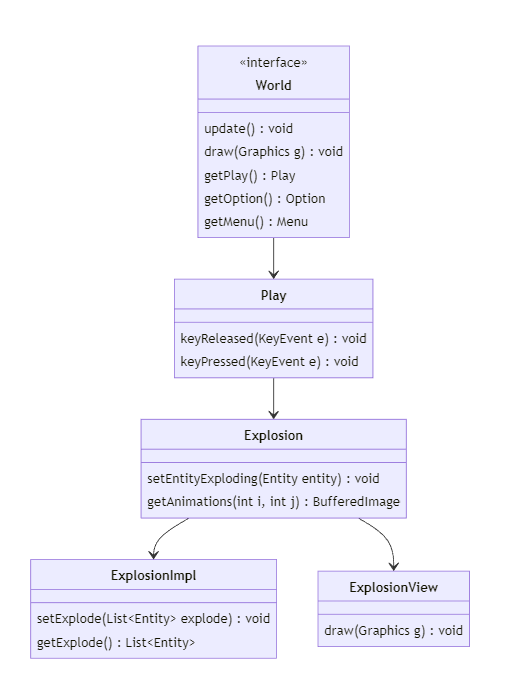
\includegraphics[width=\textwidth]{img/UMLExplosion.png}
    \caption{UML struttura MVC per le esplosioni}
\end{figure}

\paragraph{Problema} Durante l'esperienza di gioco, per una migliore user experience, dovrà essere visibile la fiammata delle esplosioni le quali vengono gestite dal proprio component (ExplodeComponent).

\paragraph{Soluzione} Per la realizzazione grafica delle esplosioni sono andato, secondo il pattern MVC, ad affidare la gestione ad un controller. Il controller di gioco (Play) ad ogni update logico dell'applicazione controlla se è presente una bomba che sta esplodendo; nel caso in cui venga trovata verrà interpellato il controller delle esplosioni il quale provvedera ad aggioranre la lista delle esplosioni presente nel Model (ExplosionImp). Successivamente la lista verrà passata alla view la quale provvederà a stamparla graficamente. Come per i model precedenti, gli sprites delle explosioni vengono caricate in fase di inizializzaione in un buffer per evitare un rallentamento successivo dell'applicazione. Gli sprites verrano caricati sotto forma di matrice dove ogni riga corrisponde alla potenza della fiammata, mentre invece ogni colonna corrisponde alla direzione della fiammata. Gestendo in questo modo le esplosioni posso distaccare completamente quello che è l'update logico della partita dall'update delle esplosioni rendendo separate le due attività. 
\subsubsection{Gestione del schermate di Pausa-Win-Lose}

\begin{figure}[H]
    \centering{}
    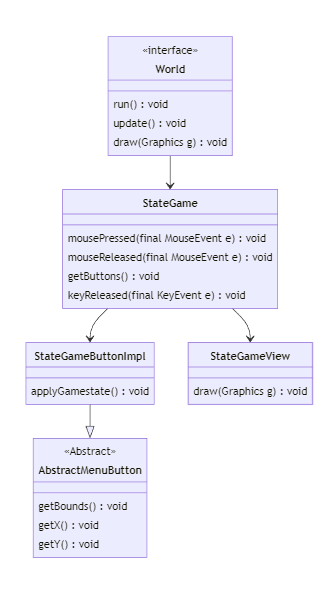
\includegraphics[width=0.75\textwidth]{img/UMLSchermatePWL.png}
    \caption{UML struttura MVC per schermate di Pause, Win, Lose}
\end{figure}

\paragraph{Problema} Durante l’esperienza di gioco dovrà essere possibile poter mettere in pausa fermando quello che che il ciclo del gioco. Inoltre arrivati a fine partita l’utente dovrà essere avvisato graficamente se ha vinto o meno quella partita.

\paragraph{Soluzione} Per la gestione della schermata di pausa, win, lose sono andato ad utilizzare un Controller unico il quale in base al Gamestate caricava la view con i bottoni corretti; andando a cambiare il press event del bottone. In questo modo se l’utente era in una situazione di pausa venivano caricati i bottoni che ti permettevano o di continuare la partita o tornare al menu; altrimenti, in situazione di win o di lose, é possibile o tornare al menu o chiudere l’applicazione con l’utilizzo dei medesimi bottoni. In questo modo ho evitato una ripetizione del codice inutile in quanto la schermata caricata graficamente era la medesima. Per la gestione della pausa mi sono affidato al keypress event il quale, nel caso in cui venisse premuto il ESC cambia il game state del gioco in PAUSE e successivamente il controller centrale, ovvero World, andrà a caricare graficamente la schermata di pausa mentre fermare update logico della partita.

\subsubsection{Gestione dell KeyInput e MouseInput}
\begin{figure}[H]
    \centering{}
    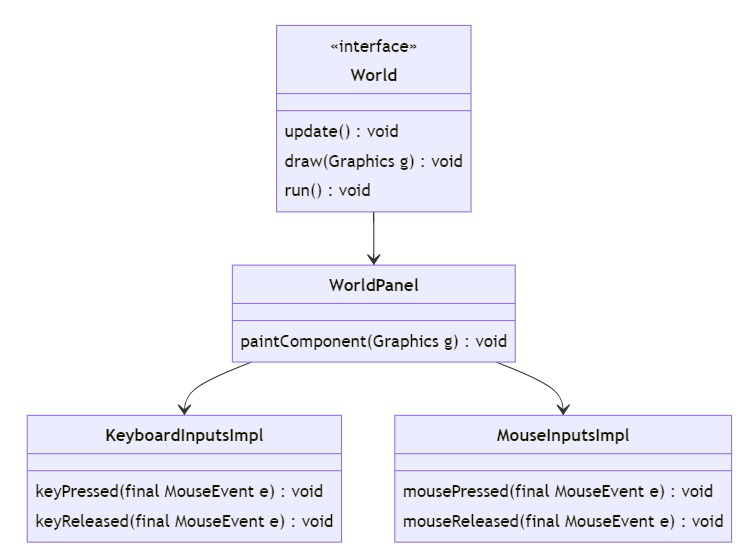
\includegraphics[width=0.75\textwidth]{img/UMLGestioneInput.png}
    \caption{UML struttura per la gestione degli input}
\end{figure}
\paragraph{Problema} Per controllare il gioco occorre avere un Handler sugli eventi del click del mouse e tastiera e indirizzare al controller corretto l’azione da effettuare. 
\paragraph{Soluzione} Per la gestione degli input da tastiera e mouse mi sono creato un handler per i KeyInput e i MouseInput. Le due classi sono state strutturate similmente. Entrambi gli handler si basano sugli eventi forniti da java.awt KeyListener e MouseListener. Questi handler non fanno altro che indirizzare al controller corretto l’evento avvenuto. In questo modo vengono interpellati solo i controller interessati mentre gli altri rimangono in attesa di futuri eventi; questo evita quindi dei rallentamenti e appesantimenti di chiamate superflue.

\chapter{Sviluppo}
\section{Testing automatizzato}
Per i test automatici, è stato utilizzato JUnit 5.
Nello specifico, i test fatti sono:
\begin{itemize}
    \item \textbf{BombTest}, il quale controlla il corretto piazzamento della bomba da parte del player e la conseguente esplosione.
    \item \textbf{BomberTest}, il quale controlla la corretta creazione del player e il suo movimento nel campo.
    \item \textbf{CollisionTest}, il quale controlla la corretta interazione tra le varie entità, le quali creano collisioni.
    \item \textbf{GameTest}, il quale controlla la corretta esecuzione delle tre fasi di gioco (partita in corso, vittoria e sconfitta).
    \item \textbf{PowerUpTest}, il quale controlla la corretta interazione tra il player e i vari tipi di power up disponibili come Bomb up e down (modifica il numero di bombe che può piazzare il player), Fire up, down e full (modifica la potenza di fuoco delle bombe piazzate), Speed up e down (modifica la velocità del player) e Throw bomb (abilita il player a lanciare le bombe)
    \item \textbf{WallTest}, il quale controlla la corretta creazione dei muri distruttibili e indistruttibili, oltre che la corretta distruzione dei primi.
\end{itemize}


\section{Metodologia di lavoro}

Innanzitutto, abbiamo iniziato con una fase di analisi dei domini e di impostazione dell'architettura da utilizzare, in modo poi di partire con lo sviluppo in maniera organizzata e precisa.
\\
Inoltre, questa fase iniziale ci ha permesso poi di lavorare per la maggior parte del tempo in maniera autonoma e parallela tra di noi, salvo dei momenti di riunione per fare i vari punti della situazione e legare i lavori individuali tra loro.
\\
Per quanto riguarda il DVCS, abbiamo optato per un utilizzo semplice come quello mostrato in classe e laboratorio, creando un repository comune che poi è stato clonato da ogni membro del gruppo nella propria macchina, consentendo così la coordinazione di tutti tramite i comandi di pull e push dei vari commit fatti.


\subsection*{Moretti Riccardo}
In autonomia mi sono occupato di:
\begin{itemize}
    \item Realizzazione delle strutture iniziali quali Entity, Component, dell’enum Type e le relative implementazioni (package it.unibo.unibomber.game.ecs.api).
    \item Realizzazione di AbstractComponent che va a generalizzare i metodi utilizzati da pressochè ogni componente package (it.unibo.unibomber.game.model.impl).
    \item Realizzazione dell’ AIComponent (package it.unibo.unibomber.game.ecs.impl).
    \item Realizzazione della movementComponent(package it.unibo.unibomber.game.ecs.impl).
    \item Realizzazione della RaisingComponent (package it.unibo.unibomber.game.ecs.impl).
    \item Realizzazione della EntityFactory (package it.unibo.unibomber.game.model.api) e relativa implementazione (package it.unibo.unibomber.game.model.impl)
    \item Realizzazione del TimesUp Component (package it.unibo.unibomber.game.model.api) e della relativa implementazione (package it.unibo.unibomber.game.model.impl)
    \item Realizzazione dell’enum Directions (package it.unibo.unibomber.utilities).
    \item Realizzazione della classe Utilities che offre diverse funzioni statiche di utilità generale (package it.unibo.unibomber.utilities).
\end{itemize}
In collaborazione mi sono occupato:
\begin{itemize}
    \item Alleggerimento della gestione delle collisioni tramite la classe Extension, che permette a entità specifiche di avere relative regole di collisione senza obbligare lo stesso codice ad entità che non ne giovano.
    \item Messa a punto della gestione
          dell’input da tastiera in keyBoardInputImpl (package it.unibo.unibomber.inputs)
\end{itemize}

\subsection*{Tamagnini Alex}
In autonomia mi sono occupato di:
\begin{itemize}
    \item Gestione dell’entità power up in PowerUpType (package it.unibo.unibomber.game.ecs.api) 
        \\e PowerUpComponent (package it.unibo.unibomber.game.ecs.impl)
    \item Gestione degli attributi dei power up legati alla bomba e al bomber in PowerUpListComponent e PowerUpHandlerComponent (package it.unibo.unibomber.game.ecs.impl)
    \item Gestione del piazzamento della bomba in BombPlaceComponent (package it.unibo.unibomber.game.ecs.impl)
    \item Gestione del calcio della bomba in SlidingComponent
          \\(package it.unibo.unibomber.game.ecs.impl)
    \item Gestione del lancio della bomba in ThrowComponent 
    \\(package it.unibo.unibomber.game.ecs.impl)
    \item Creazione dei test, tra cui:
          \begin{itemize}
              \item PowerUpTest (package it.unibo.unibomber.model)
              \item BomberTest (package it.unibo.unibomber.model)
              \item testBombPlace in BombTest (package it.unibo.unibomber.model)
          \end{itemize}
\end{itemize}
In collaborazione, mi sono occupato di:
\begin{itemize}
    \item Implementazioni di controlli relativi a collisioni tra bomber e power up, e tra bomber e bomba con power up KICKBOMB in CollisionComponent (package it.unibo.unibomber.game.ecs.impl) ed in Extension (package it.unibo.unibomber.game.model.impl)
    \item Inserimento di alcune costanti in Constants 
    \\(package it.unibo.unibomber.utilities)
    \item Inserimento di alcuni metodi, utilizzati da più classi, in Utilities (package it.unibo.unibomber.utilities)
    \item Implementazione di alcuni controlli riguardanti il power up KICKBOMB in testCollisionsPlayerBombSliding in CollisionTest (package it.unibo.unibomber.model)
\end{itemize}

\subsection*{Bertozzi Niccolò}
In autonomia mi sono occupato di:
\begin{itemize}
    \item Gestione del GameLoop in GameLoop 
        \\(package it.unibo.unibomber.controller.api) e WordImpl 
        \\(package it.unibo.unibomber.controller.impl)
    \item Creazione della Windows iniziale andando a ridimensionare le sites dei vari componenti grafici in base alla risoluzione dello schermo utilizzato (package it.unibo.unibomber.view)
    \item Gestione del Keyinput e MouseInput 
    \\(package it.unibo.unibomber.inputs)
    \item Gestione delle collisione tra le varie entità in CollisionComponent 
    \\(package it.unibo.unibomber.game.ecs.impl) e Extension 
    \\(package it.unibo.unibomber.game.model.impl)
    \item Gestione della grafica del menu in Menu 
    \\(package it.unibo.unibomber.controller.impl), MenuButtonImpl 
    \\(package it.unibo.unibomber.game.model.impl) e MenuView 
    \\(package it.unibo.unibomber.view)
    \item Gestione della grafica delle opzioni in Option 
    \\(package it.unibo.unibomber.controller.impl), OptionButtonImpl 
    \\(package it.unibo.unibomber.game.model.impl), OptionView
    \\(package it.unibo.unibomber.view) e HandicapView 
    \\(package it.unibo.unibomber.view)
    \item Gestione della grafica della partita in Play 
    \\(package it.unibo.unibomber.controller.impl), PlayImpl 
    \\(package it.unibo.unibomber.game.model.impl) e PlayView 
    \\(package it.unibo.unibomber.view)
    \item Gestione della grafica delle esplosioni a livello grafico  in Explosion 
    \\(package it.unibo.unibomber.controller.impl), ExplosionImpl 
    \\(package it.unibo.unibomber.game.model.impl) e ExplosionView 
    \\(package it.unibo.unibomber.view)
    \item Gestione della grafica degli stati del gioco (Pause, Victory, Lose) in StateGame (package it.unibo.unibomber.controller.impl), StateGameButtonImpl (package it.unibo.unibomber.game.model.impl) e StateGameView (package it.unibo.unibomber.view)
    \item Realizzazione dei test relativi alle Collisioni e al TimesUp  (package it.unibo.unibomber.model).
\end{itemize}
In collaborazione mi sono occupato di:
\begin{itemize}
    \item Alleggerire la struttura delle collisioni tramite Extension 
    \\(package it.unibo.unibomber.game.model.impl).
    \item Implementazione del Times Up finale.
    \item Gestione di un file contente tutte le costanti necessarie in Constants (package it.unibo.unibomber.utilities)
\end{itemize}


\subsection*{Rigoni Lorenzo}
In autonomia mi sono occupato di:
\begin{itemize}
    \item Gestione della distruzione di un’entità con il DestroyComponent (package it.unibo.unibomber.game.ecs.impl)
    \item Gestione della esplosione della bomba con l’ExplodeComponent (package it.unibo.unibomber.game.ecs.impl)
    \item Creazione dell’interfaccia Field
        \\(package it.unibo.unibomber.game.model.api)
    \item Creazione dei test, tra cui:
          \begin{itemize}
              \item WallTest (package it.unibo.unibomber.model)
              \item GameTest (package it.unibo.unibomber.model)
              \item testBombExplosion in BombTest 
              \\(package it.unibo.unibomber.model)
          \end{itemize}
\end{itemize}
In collaborazione, mi sono occupato di:
\begin{itemize}
    \item Implementazione dell’interfaccia Field in FieldImpl con Moretti Riccardo (package  it.unibo.unibomber.game.model.impl)
\end{itemize}
\subsection*{Lavoro in gruppo:}
\begin{itemize}
    \item Gestire la generazione delle singole entità in EntityFactoryImpl (package it.unibo.unibomber.game.model.impl)
    \item Gestione di un file contente tutte le costanti necessarie in Constants (package it.unibo.unibomber.utilities)
    \item Gestione utilities
\end{itemize}

\section{Note di sviluppo}
\subsection*{Moretti Riccardo}

\subsection*{Tamagnini Alex}

\subsection*{Bertozzi Niccolò}
\subsubsection*{Utilizzo di Stream e lambda expressions:}
\begin{itemize}
    \item Permalink: 
    \\ \url{https://github.com/TamagniniAlex/OOP22-unibomber/blob/84d383be9de179a92d9b3358ab2a3eb2b514631d/src/main/java/it/unibo/unibomber/controller/impl/Play.java#L61-L67}
    \item Permalink: 
    \\ \url{https://github.com/TamagniniAlex/OOP22-unibomber/blob/84d383be9de179a92d9b3358ab2a3eb2b514631d/src/main/java/it/unibo/unibomber/game/ecs/impl/CollisionComponent.java#L101-L106}
    \item Permalink: 
    \\ \url{https://github.com/TamagniniAlex/OOP22-unibomber/blob/84d383be9de179a92d9b3358ab2a3eb2b514631d/src/main/java/it/unibo/unibomber/game/model/impl/Extension.java#L127-L134}
    \item Permalink: 
    \\ \url{https://github.com/TamagniniAlex/OOP22-unibomber/blob/84d383be9de179a92d9b3358ab2a3eb2b514631d/src/main/java/it/unibo/unibomber/controller/impl/Play.java#L61-L67}
    \item Permalink: 
    \\ \url{https://github.com/TamagniniAlex/OOP22-unibomber/blob/84d383be9de179a92d9b3358ab2a3eb2b514631d/src/test/java/it/unibo/unibomber/model/WallTest.java#L81-L82}
\end{itemize}
\subsubsection*{Utilizzo di Optional:}
\begin{itemize}
    \item Permalink: \url{https://github.com/TamagniniAlex/OOP22-unibomber/blob/main/src/main/java/it/unibo/unibomber/controller/impl/StateGame.java#L52-L54}
\end{itemize}
\subsection*{Rigoni Lorenzo}
\subsubsection*{Utilizzo di Stream e lambda expressions:}
\begin{itemize}
    \item Permalink: 
    \\ \url{https://github.com/TamagniniAlex/OOP22-unibomber/blob/main/src/main/java/it/unibo/unibomber/game/ecs/impl/DestroyComponent.java#L117-L121}
    \item Permalink: 
    \\\url{https://github.com/TamagniniAlex/OOP22-unibomber/blob/main/src/main/java/it/unibo/unibomber/game/ecs/impl/DestroyComponent.java#L150-L153}
    \item Permalink: 
    \\\url{https://github.com/TamagniniAlex/OOP22-unibomber/blob/main/src/main/java/it/unibo/unibomber/game/ecs/impl/ExplodeComponent.java#L167-L170}
    \item Permalink: 
    \\\url{https://github.com/TamagniniAlex/OOP22-unibomber/blob/main/src/main/java/it/unibo/unibomber/game/ecs/impl/ExplodeComponent.java#L207-L209}
\end{itemize}
\subsubsection*{Utilizzo di Optional:}
\begin{itemize}
    \item Permalink: \url{https://github.com/TamagniniAlex/OOP22-unibomber/blob/main/src/main/java/it/unibo/unibomber/game/ecs/impl/ExplodeComponent.java#L199-L210}
\end{itemize}

\chapter{Commenti finali}

\section{Autovalutazione e lavori futuri}
\subsection*{Moretti Riccardo}

\subsection*{Tamagnini Alex}
Lavorare per questo progetto è stato soddisfacente ed interessante in quanto, lavorando molto bene in gruppo, siamo riusciti a sviluppare un videogioco partendo da zero utilizzando anche tecniche di programmazione che non conoscevo. Ci siamo impegnati al massimo, e penso che il nostro lavoro sia stato valido.
Come autovalutazione, mi darei un voto più che sufficiente, dato che sono riuscito a seguire le scadenze senza troppa difficoltà, anche se potrei migliorare la capacità di sviluppare un programma con l'idea di estendibilità fin da subito.
Ho apprezzato molto la possibilità di lavorare in gruppo e di confrontarmi con gli altri membri del team. Ritengo che complessivamente questo progetto sia stato una grande opportunità di crescita personale e professionale, permettendomi di migliorare le mie competenze in Java e di essere maggiormente confacente ai miei obiettivi nel futuro oltre ad essere orgoglioso dei risultati raggiunti insieme alla mia squadra.
Infine per quanto riguarda i lavori futuri sarebbe molto interessante estendere il progetto aggiungendo nuove funzionalità e migliorando quelle già presenti.

\subsection*{Bertozzi Niccolò}
La realizzazione di questo progetto di gruppo è stata un'esperienza molto gratificante e formativa per tutti noi. Abbiamo lavorato sodo per mesi, affrontando insieme sfide tecniche e di team working, e alla fine siamo riusciti a creare un gioco divertente e coinvolgente.
Dal punto di vista dell'autovalutazione, credo che il nostro gruppo abbia fatto un buon lavoro nel definire le specifiche del gioco e nell'implementare in Java, sfruttando le nostre conoscenze e competenze informatiche. Inoltre, abbiamo lavorato bene insieme, comunicando in modo chiaro e costruttivo e facendo fronte alle difficoltà con determinazione e collaborazione.
Tuttavia, penso che ci sarebbe stato spazio per migliorare alcuni aspetti del nostro lavoro. Ad esempio, avremmo potuto dedicare più tempo alla progettazione dell'interfaccia grafica, che in alcuni punti risulta un po' grezza, o organizzare meglio le fasi di testing per evitare di incorrere in bug o problemi inaspettati.
Per quanto riguarda i progetti futuri, credo che sarebbe interessante continuare a lavorare su questo gioco, magari estendendolo con nuove funzionalità o ambientazioni, o provare a creare un nuovo gioco partendo da zero. In ogni caso, penso che questa esperienza ci abbia permesso di crescere come programmatori e come team, e non vedo l'ora di mettere le nostre competenze in pratica anche in futuro.

\subsection*{Rigoni Lorenzo}
Sono felice e soddisfatto del progetto svolto, in quanto mi ha aiutato a comprendere maggiormente la programmazione ad oggetti e le opportunità che ti può offrire un linguaggio ad alto livello come Java. Inoltre, mi sono trovato bene a lavorare insieme a questo gruppo con cui mi sono subito trovato in sintonia, sia dal punto di vista lavorativo sia dal punto di vista umano. Nonostante l’inesperienza nella creazione di un gioco, questo progetto mi ha dato delle solide basi e mi piacerebbe crearne di nuovi in futuro.

\appendix
\chapter{Guida utente}

All’avvio del gioco, si potrà scegliere la mappa in cui giocare, il numero di bot contro cui giocare (da 1 a 3) andando ad aumentare (+) o diminuire (-); e la possibilità di mettere dei power up iniziali al player e/o ai bot.
\\
\\
Per quanto riguarda i comandi di gioco durante la partita, sono i seguenti:
\begin{itemize}
    \item \textbf{ESC} (Escape): Il gioco va in pausa e si può scegliere se continuare la partita (Continue) o uscire (Quit).
    \item \textbf{W}: Movimento verso l'alto.
    \item \textbf{A}: Movimento verso sinistra.
    \item \textbf{S}: Movimento verso il basso.
    \item \textbf{D}: movimento verso destra
    \item \textbf{SPACE} : Piazza la bomba.
    \item \textbf{E}: Lancia la bomba (avendo preso il power up “Throw bomb”, ovvero il pugno blu).
\end{itemize}

\bibliographystyle{alpha}
\bibliography{report}
\begin{itemize}
    \item Per gli sprites relativi al bomber e le sue animazioni  \url{https://www.spriters-resource.com/ds_dsi/bomberman/sheet/7999/}
    \item Per gli sprites relativi alle bombe \url{https://www.spriters-resource.com/ds_dsi/bomberman/sheet/107788/?source=genre}
    \item Sprites mappa \url{https://www.spriters-resource.com/ds_dsi/bomberman/sheet/108163/} e \url{https://www.spriters-resource.com/ds_dsi/bomberman/sheet/114393/}
\end{itemize}
\end{document}
